\documentclass[a4paper, 10pt, final, garamond]{book}
\usepackage{cours-preambule}
\usepackage{pdfpages}

\raggedbottom

\makeatletter
\renewcommand{\@chapapp}{Travaux pratiques -- TP}
\makeatother

\let\SavedIndent\indent
\protected\def\indent{%
  \begingroup
    \parindent=\the\parindent
    \SavedIndent
  \endgroup
}
\setlength{\parindent}{0pt}

\begin{document}
\setcounter{chapter}{20}

\chapter{Dosage par titrage acidobasique avec suivi pH-m\'etrique et
conductim\'etrique du vinaigre}

\section{Objectifs}

\begin{itemize}
    \item Revoir le protocole de dilution.
    \item Revoir le protocole expérimental de pH-métrie~; Tracer des courbes 
        pH-métriques grâce à Régressi ou Latispro.
    \item Choisir un indicateur coloré acido-basique.
    \item Comprendre le principe de la conductimétrie et connaître les formules.
    \item Revoir le protocole expérimental de conductimétrie~; Tracer des
        courbes conductimétriques grâce à Régressi ou Latispro.
    \item Exploiter une équivalence pour déterminer le degré alcoolique d'un
        vinaigre.
    \item Évaluer une incertitude lors de mesures avec des appareils de
        tolérance connue.
    \item Évaluer une incertitude de mesure dans laquelle interviennent
        plusieurs sources d'erreurs.
\end{itemize}

\section{S'approprier}
\subsection{Introduction}

On cherche à déterminer le degré d'un vinaigre par titrage pH-métrique et
conductimétrique, à partir d'une solution d'hydroxyde de sodium (soude)
(\ce{Na+}~; \ce{OH-}). Un vinaigre est essentiellement une solution aqueuse
diluée d'acide éthanoïque (ou acétique) de formule \ce{CH3COOH}. Les
concentrations commerciales sont exprimées en degrés. Le degré d'un vinaigre
correspond à la masse (en gramme) d'acide éthanoïque pur contenu dans
$\SI{100}{g}$ de vinaigre.

\subsection{Données utiles}

\begin{itemize}
    \item Masses molaires~: $M(\ce{H}) = \SI{1,0}{g.mol^{-1}}$, $M(\ce{O}) =
        \SI{16,0}{g.mol^{-1}}$ et $M(\ce{C}) = \SI{12,0}{g.mol^{-1}}$
    \item Masse volumique du vinaigre~: $\rho_V \approx \SI{1,0}{g.cm^{-3}}$
    \item Couples acido-basiques mis en jeu~: \ce{H2O/OH-} (pK$_A = 14$) et
        \ce{CH3COOH/CH3COO-} de pK$_A = \num{4,8}$.
\end{itemize}

\subsection{Principe d'un pH-mètre}

Un pH-mètre est constitué de deux électrodes~: une électrode de verre de
potentiel d'électrode proportionnel au pH de la solution dans laquelle elle
trempe et une électrode de référence (pour laquelle le potentiel d'électrode est
fixe). Ces deux électrodes constituent une pile électrochimique et un
millivoltmètre mesure la force électromotrice $e$ de cette pile, qui est une
fonction affine du pH~: $e = a + b \rm pH$ où $a$ et $b$ sont deux constantes
qui dépendent de la nature des électrodes et de la température.  Avant toute
mesure, il faut donc étalonner le pH-mètre.

\subsection{Le principe de la conductimétrie}

Cette méthode repose sur l'existence d'ions en solution et sur leur capacité à
faciliter le passage d'un courant. La nature des ions et leurs concentrations
modifient la conductance $G$ du système (grandeur qui est l'inverse de la
résistance $R$) exprimée en \si{S} (Siemens). Plus le milieu est propice au
passage du courant, plus la conductance est élevée. Celle-ci est reliée à trois
paramètres principaux~:

\begin{enumerate}
    \item la conductivité $\sigma$ du système
    \item la longueur $\ell$
    \item la section $S$ de la cellule
\end{enumerate}

La conductance s'exprime alors selon
\[G = \frac{\sigma S}{\ell}\]

Ainsi, on ne parle pas de conductance \cancel{de la solution}, puisque la
conductance dépend de la cellule de mesure et de sa géométrie. L'unité de
conductivité est le $\si{S.m^{-1}}$~; le quotient $K = \ell / S$ est appelé
constante de cellule. Ainsi, on a $G = \sigma / K$. La mesure de la conductance
s'effectue avec un conductimètre, qui est en fait un ohmmètre.\bigbreak

La conductivité $\sigma$ de la solution peut alors s'exprimer par la \textbf{loi
de Kohlrausch}, exprimée sous une forme avec la chage de l'ion~:
\begin{tprop}{Loi de \textsc{Kohlrausch}}
    \[\boxed{\sigma = \sum_{i} \lambda_i \left|z_i\right| [{\rm X}_i]}\]

    Avec~:
    \begin{itemize}
        \item $\lambda_i$ la conductivité molaire ionique de l'ion ${\rm X}_i$ (en
            $\si{S.m^2.mol^{-1}}$) donnée dans les tables
        \item $z_i$ la charge de l'ion ${\rm X}_i$
        \item $[{\rm X}_i]$ la concentration de l'ion ${\rm X}_i$ en
            $\si{mol.m^{-3}}$ (\textbf{Attention~!!})
    \end{itemize}
\end{tprop}

\begin{rror}{Important}
    \begin{center}
        \bfseries
        La conductivité $\sigma$ de la solution prend en compte tous les ions
        présents dans la solution. Il faut donc faire l'inventaire des ions en
        solution avec soin, y compris les ions spectateurs.
    \end{center}
    La conductivité $\sigma$ évoluera donc lorsque la concentration des ions
    changera \textbf{ou} lorsque leur nature (et donc leur conductivité molaire
    ionique) changera. Et si le volume total de la solution peut être considéré
    constant, $\sigma$ sera une \textbf{fonction affine du volume versé lors
    d'un dosage}, la pente étant fonction des conductivités molaire ionique de
    chacun des ions qui apparaissent/disparaissent. \textbf{C'est pourquoi, on
    réalisera ce dosage avec un excès d'eau distillée}, pour pouvoir supposer le
    volume invariant par apport de solution titrante.
\end{rror}

\section{Analyser}
\subsection{Étude générale du dosage}

\vspace{-10pt}
\begin{minipage}{0.75\linewidth}
    \begin{enumerate}[label=\clenumi]
        \item Écrire l'équation du dosage, calculer la constante de la réaction
            en fonction des pK$_A$ et conclure sur la pertinence (est-elle
            totale~?) de cette réaction comme réaction de dosage.
        \item Pourquoi peut-on suivre ce dosage par pH-métrie~? par
            conductimétrie~?
        \item Sur l'étiquette de la bouteille de soude caustique, on peut voir
            ce pictogramme~: que signifie-t-il~? Quelles précautions faut-il
            prendre~? 
    \end{enumerate}
    Vous pourrez consulter \url{http://www.inrs.fr/media.html?refINRS=ED%204406}
\end{minipage}
\hfill
\begin{minipage}{0.20\linewidth}
    \begin{center}
        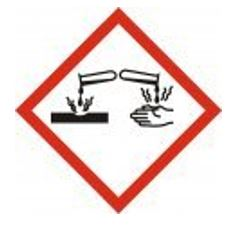
\includegraphics[width=\linewidth]{ch21picto}
    \end{center} 
\end{minipage}

\subsection{Préparation de la solution $S_1$ à doser}

On souhaite doser $V_A = \SI{10}{mL}$ de vinaigre à partir d'une solution
d'hydroxyde de sodium ou soude de formulation une fois dissociée dans l'eau 
(\ce{Na+}~; \ce{HO-}) et de concentration $C_B = \SI{1,0e-1}{mol.L^{-1}}$. On
utilisera la burette sortie sur la paillasse ($\SI{25}{mL}$).

\bigbreak

\begin{enumerate}[label=\clenumi, resume]
    \item Le vinaigre que nous utilisons a un degré alcoolique de 8. Peut-on
        utiliser directement la solution commerciale ou faut-il la diluer~? Si
        oui dans quelles proportions~? Expliquer, dans ce cas, votre protocole
        expérimental.
\end{enumerate}

\section{Réaliser}

\begin{bror}{Important}
    \begin{center}
        \bfseries
        Le port de la blouse fermée et des lunettes est obligatoire durant
        l'ensemble du TP. Les cheveux longs doivent être attachés, les lentilles
        de contact retirées.
    \end{center}
\end{bror}

\subsection{Préparation de la solution $S_1$ à doser}

\begin{itemize}[label=$\triangleright$]
    \item Préparer la solution $S_1$ selon le protocole que vous avez établi
        dans la partie Analyser. 
\end{itemize}

\subsection{Réalisation du dosage par pH-métrie}

\begin{bror}{Important}
    \begin{center}
        \bfseries
        Attention, une sonde pH-métrique est très fragile (et très couteuse).
        Merci de manipuler avec beaucoup de précaution.
    \end{center}
\end{bror}

\subsubsection{Étalonnage du pH-mètre}

\begin{enumerate}
    \item La relation étant supposée linéaire (\textit{cf} S'approprier), il
        suffit d'utiliser deux solutions étalon (solutions tampons à pH fixé)
        afin d'avoir deux points de contrôle (une droite est définie avec
        unicité par la connaissance de deux points). Le protocole est affiché
        dans la salle en fonction des pH-mètres présents.
    \item Enlever les caches des électrodes et les rincer à l'eau distillée.
    \item Appuyer sur \texttt{cal}.
    \item Tremper les électrodes dans la solution pH = 7, puis à l'aide des
        flèches, amener la valeur du pH sur 7, avant de valider. Certains
        modèles s'autocalibrent, dans ce cas il suffit d'attendre. 
    \item Rincer les électrodes entre les deux solutions tampon.
    \item Recommencer avec la 2\ieme\ solution tampon à pH = 4.
    \item Rincer de nouveau à l'eau distillée, puis appuyer sur mesure.
    \item Le pH-mètre est prêt à être utilisé~!
\end{enumerate}

\subsubsection{Dosage}

\begin{enumerate}
    \item Remplir la burette avec la solution de soude. Purger la partie basse
        de la burette (éliminer les éventuelles bulles d'air) et ajuster le zéro
        de la burette. Il est impératif que la partie basse de la burette
        contienne de la solution titrante, sinon vos mesures vont être erronées. 
    \item Rincer la pipette avec la solution $S_1$ de vinaigre préparée, puis
        prélever $\SI{10}{mL}$ de cette solution et la mettre dans le bécher.
        Ajouter environ $\SI{30}{mL}$ d'eau distillée de façon à ce que les
        électrodes puissent tremper.
    \item Placer les électrodes de mesures dans le bécher et mettre l'agitation
        magnétique en marche. \textbf{Attention, le barreau magnétique ne doit
        pas toucher les électrodes}.
\end{enumerate}
\begin{enumerate}[label=\sqenumi, start=5]
    \item Faire le schéma du montage sur votre compte-rendu.
    \item Réaliser les mesures en remplissant un tableau de valeurs permettant
        de tracer $\pH = f(V_B)$, pour des additions de soude de $0,1,2… \si{mL}$
        jusqu'à ce que $V_B \approx 2 V_{Beq}$.
\end{enumerate}

\subsubsection{Exploitation des mesures}

\begin{enumerate}
    \item Allumer l'ordinateur sur votre session, puis ouvrir Régressi.
    \item Aller dans Fichier, nouveau, clavier et recopier votre tableau de
        valeurs $(V_B~; \pH)$.
    \item Afficher le graphe $\pH = f(V_B)$. Relier les points expérimentaux
        grâce aux options de graphe et réaliser un lissage d'ordre 3.
    \item Afin de déterminer l'équivalence, Regressi comporte directement la
        méthode des tangentes. Dans le menu graphique, allez dans Outils
        $\rightarrow$ tangente $\rightarrow$ méthode des tangentes (avec clic)
        $\rightarrow$ cliquez sur un point juste avant ou juste après
        l'équivalence. 
\end{enumerate}
\begin{enumerate}[label=\sqenumi, start=7]
    \item Imprimer la courbe et relever le volume de soude versé à
        l'équivalence~: $V_{Beq}$.
    \item Donner la relation à l'équivalence. On notera $C_1$ la concentration
        en acide acétique du vinaigre dilué de la solution $S_1$. En déduire la
        concentration $C_A$ de la solution commerciale.
    \item Calculer l'écart relatif sur la concentration commerciale.
\end{enumerate}

\subsection{Dosage pH-métrique par suivi colorimétrique~: choix de l'indicateur}

Les indicateurs colorés de pH (ou indicateurs acide-base) sont des molécules qui ont la capacité de changer de couleur en fonction de l'acidité de leur milieu environnant.

\begin{timpo}{Rappel}
    La zone de virage de l'indicateur coloré doit contenir le pH à l'équivalence
    $\pH\ind{eq}$. Ainsi, lors du saut de $\pH$ consécutif au changement de
    réactif limitant, il y a changement franc de la couleur de l'indicateur. 
\end{timpo}

\begin{table}[h!]
    \centering
    \caption{Indicateurs proposés.}
    \label{tab:ind}
    \begin{tabular}{lccc}
        \toprule
        Indicateur & Couleur acide & Zone de virage & Couleur basique
        \\\midrule
        Bleu de bromothymol & jaune & \SIrange{6.0}{7.6}{} & bleu
        \\
        Rouge de crésol & jaune & \SIrange{7.2}{8.1}{} & rouge
        \\
        Hélianthine & rouge & \SIrange{3.2}{4.4}{} & jaune
        \\\bottomrule
    \end{tabular}
\end{table}

\begin{enumerate}[label=\sqenumi, resume]
    \item Parmi les indicateurs de la table~\ref{tab:ind}, quel indicateur
        coloré faudrait-il choisir pour réaliser un dosage colorimétrique du
        vinaigre~? 
\end{enumerate}

\begin{bror}{Important}
    \begin{center}
        \bfseries
        Nous ne réaliserons pas ce dosage.
    \end{center}
\end{bror}

\subsection{Réalisation du dosage par conductimétrie}
\subsubsection{Préparation du conductimètre}

La cellule conductimétrique est constituée de deux lames planes, parallèles, en
platine platiné (platine recouvert de platine par hydrolyse). Le conductimètre
mesure la résistance $R$ ou la conductance $G$ de la colonne de solution qui est
directement proportionnelle à la conductance $\sigma$. La cellule du
conductimètre est conservée dans un grand bécher contenant de l'eau distillée,
il ne reste plus qu'à la plonger dans la solution à étudier. 

\subsubsection{Dosage}

\begin{enumerate}
    \item Suivre le même protocole que pour le dosage pH métrique. 
    \item Mettre les $\SI{10}{mL}$ de la solution $S_1$ préalablement préparée
        dans un grand bécher et ajouter de $200$ à $\SI{250}{mL}$ d'eau
        distillée (la précision du volume n'a aucune importance tant qu'il est
        suffisant pour pouvoir négliger le volume de solution titrante versé).
\end{enumerate}
\begin{enumerate}[label=\sqenumi, start=11]
    \item Réaliser les mesures en remplissant un tableau de valeurs permettant
        de tracer $G = f (V_B)$, pour des additions de soude de $0,1,2… \si{mL}$
        jusqu'à ce que $V_B \approx 2 V_{Beq}$.
\end{enumerate}

\subsubsection{Exploitation des mesures}

Connectez-vous sur \texttt{Capytale} à l'adresse \url{https://capytale2.ac-paris.fr/web/c/cf5a-1487558}, puis~:

\begin{enumerate}
    \item Compléter les listes $V$, $G$ de vos valeurs relevées. 
    \item Tracer le nuage de points.
    \item Créer les listes de points correspondant aux points avant et après
        l'équivalence et les tracer sur le graphe correspondant.
    \item Calculez les paramètres des fonctions affines par morceaux ainsi
        définies, et les tracer.
    \item Relever à l'aide de la souris le volume de soude
        versé à l'équivalence~: $V_{Beq}$ (comme étant l'intersection des
        modélisations affines), et rentrer sa valeur dans la cellule
        correspondante.
    \item En déduire la concentration $C_1$ en acide acétique de la solution
        $S_1$, puis la concentration $C_A$ de la solution commerciale.
    \item En déduire le degré alcoolique expérimental du vinaigre.
    \item Calculer l'écart relatif.
\end{enumerate}

\section{Valider~: évaluation des incertitudes de mesures}

L'objectif est de déterminer l'incertitude-type sur la grandeur $C_1$, que l'on
notera $u(C_1)$. Cette concentration est obtenue par dosage et s'obtient d'après
l'expression 

\[
    C_1 = \frac{C_B V\ind{Beq}}{V_A}
\]

L'obtention de $u(C_1)$ va donc être réalisée en deux temps, à effectuer sur
\texttt{Capytale}~:
\begin{enumerate}
    \item Détermination de l'incertitude de type B sur les grandeurs $C_B$,
        $V\ind{Beq}$ et $V_A$. On prendra $u(C_B)/C_B \approx 1 \%$, et vous
        déterminerez les autres incertitudes.
    \item Détermination de $u(C_1)$ par propagation des incertitudes grâce à la
        méthode Monte-Carlo.
\end{enumerate}

\section{Conclure}

\begin{enumerate}[label=\sqenumi, start=12]
    \item En tenant compte des indications précédentes, calculer $u(C_1)$ et
        écrire le résultat du mesurage de $C_1$ sous la forme $M(C_1) = m(C_1)
        \pm u(C_1)$. Vous justifierez les incertitudes de type B que vous avez
        choisi pour $V\ind{Beq}$ et $V_A$.
\end{enumerate}

% \begin{programme}{}
% 
% \vspace{1cm}
% \begin{itemize}
% \item Titrage direct
% \item Equivalence
% \item Identifier  et  exploiter  la  réaction  support  du  titrage 
% (recenser les espèces présentes dans le milieu  au 
% cours   du   titrage,   repérer   l'équivalence,   justifier 
% qualitativement    l'allure    de    la    courbe    ou    le 
% changement de couleur observé). 
% \item Indicateur coloré de fin de titrage
% \item Choisir  et  utiliser  un  indicateur  coloré  de  fin  de 
% titrage. 
% \item Distinguer l'équivalence et le virage d'un indicateur 
% coloré de fin de titrage. 
% \item Exploiter  une  courbe  de  titrage  pour  déterminer  la 
% concentration d'une espèce dosée. 
% \item Titrage par suivi conductimétrique et pH-métrique
% \end{itemize}
% \end{programme}

\end{document}

